%%%%%%%%%%%%%%%%%%%%%%%%%%%%%%%%%%%%%%%%%%%%%%%%%%%%%%%%%%%%%%%%%%%%%%%%%%%%%%%
\chapter{Results}
\ifpdf
    \graphicspath{{Chapter4/Figs/Raster/}{Chapter4/Figs/PDF/}{Chapter4/Figs/}}
\else
    \graphicspath{{Chapter4/Figs/Vector/}{Chapter4/Figs/}}
\fi

This chapter examines the main results from application of \textbf{Frontier} and
\textbf{scikit-learn} to our \textbf{auto\_qc} learning task.

\section{Introduction}

To recap...

\begin{itemize}
    \item Set up environment for decision tree classification...
    \item Select an appropriate set of parameters to use...
    \item Minimise decision tree...
    \item Apply best practice..
    \item Best parameters...?
    \item Identified any parameters that match or not?
\end{itemize}

\section{Introduction}
\subsection{Why Decision Trees?}
%TODO Citations...

...each node represents a test on the value of an attribute or feature

...single discrete target
...primarily human readable rule set... like a flow chart...
...simple to interpret, can be statistically verified
...robust to noise
...realistic applications in medicine and risk
...algorithm capable of scaling to relatively large sets such as ours
...at this time we're not looking for a "black box"
...want to be able to see whether the current rule set can be extracted with
machine learning methods...

...decisions tree however are prone to overfitting -- failing to generalise...
...cannot promise optimality
...duplicated subtrees
...cannot be applied to first order logic, only one parameter can be tested at a
time, future tests are not "aware" of previous tests

\subsection{DecisionTreeClassifier}
% TODO Cite
% http://scikit-learn.org/stable/modules/generated/sklearn.tree.DecisionTreeClassifier.html
...gini impruty or information gain... scikit seems to favour gini...
...


...Classification And Regression Tree (CART)





\section{Naive Parameter Sets}
\subsection{Introduction}

For initial training and testing purposes, the following arbitrary parameter
sets were created as a starting point:

\begin{itemize}
    \item \textbf{ALL} \hfill\\
        A parameter set consisting of all the summary numbers in a "BAMcheckr'd"
        file
    \item \textbf{AQC} \hfill\\
        A set consisting of all available parameters used by \textbf{auto\_qc}.
    \item \textbf{AQCN} \hfill\\
        Replaces groups of the \textbf{AQC} set with aggregated parameters.
    \item \textbf{ERROR} \hfill\\
        An experimental toy set consisting of only the "error-rate" parameter.
    \item \textbf{NO\_ERROR} \hfill\\
        Another toy set designed to test results gained by excluding the
        "error-rate" parameter.
    \item \textbf{BASELINE} \hfill\\
        Include any parameter which includes "baseline" as a substring.
    \item \textbf{NOBASELINE} \hfill\\
        Exclude any parameter which includes "baseline" as a substring.
    \item \textbf{MARP} \hfill\\
        Include any parameter which includes any of the following as substrings:
        mean, average, rate or percent.
    \item \textbf{NO\_MARP} \hfill\\
        Exclude any parameter which includes any of the following as substrings:
        mean, average, rate or percent.
\end{itemize}

Of particular note is the \textbf{AQC} set, constructed from the parameters
available from the "BAMcheckr'd" data that are taken into account by the
current \textbf{auto\_qc} system. However not all these
parameters were initially available in the input files and \textbf{auto\_qc}
relies upon data made available from \textbf{vr-pipe} where the rules of
\textbf{auto\_qc} are actually applied; Appendix~\ref{app:ratios} discusses
contributions I made to \textbf{bamcheckr} for recovering these parameters for
use in our analysis. Ultimately, \textbf{bamcheckr} performed too slowly and it
was possible to use \textbf{Frontier} itself to extract the additional features
needed to better represent the decisions made by the current system.

\subsection{Experiment Results}
%TODO Cite dtc, skfold
For each parameter set, data and targets were extracted via \textbf{Frontier}'s
API before being subset by \textbf{scikit-learn}'s \textbf{StratifiedKFold}
function. All available data (13,455 "BAMcheckr'd" lanelets) were used as input
and the target variable could be one of three classes; pass, fail or warn.
The subsets are referred to as "folds" (of which we used 10) and for
each fold a \textbf{DecisionTreeClassifier} was trained and tested.
Table~\ref{tab:pset-cv} outlines the average cross validation scores across each
such experiment.

\begin{table}[H]
    \centering
    \begin{tabular}{l | c  c  c  c  r}
        Set           & Nº & CV ± SD & SCV ± SD & Depth & Most Important Feature\\
        \hline
        ALL           & 86 & 90 ± 4 & 97 ± 1 & 38 & T-percent-max-baseline-deviation (27\%)\\
        AQC           & 27 & 87 ± 4 & 95 ± 1 & 36 & T-percent-max-baseline-deviation (31\%)\\
        AQCN          & 21 & 86 ± 4 & 95 ± 1 & 39 & max-max-baseline-deviation (31\%)\\
        ERROR         & 1  & 60 ± 6 & 61 ± 2 & 53 & error-rate (100\%)\\
        NO\_ERROR     & 85 & 90 ± 4 & 97 ± 1 & 38 & T-percent-max-above-baseline(27\%)\\
        BASELINE      & 34 & 82 ± 5 & 89 ± 1 & 46 & T-percent-max-above-baseline(28\%)\\
        NOBASELINE    & 52 & 72 ± 10 & 91 ± 1 & 31 & error-rate (24\%)\\
        MARP          & 47 & 87 ± 4 & 95 ± 1 & 39 & T-percent-max-above-baseline (27\%)\\
        NO\_MARP      & 39 & 75 ± 7 & 87 ± 1 & 38 & max-max-baseline-deviation (34\%)\\
    \end{tabular}

    \caption[pset-cv]{\textbf{Parameter Set Cross Validation Scores}: Results of
        classifying testing data into one of three classes; pass, fail or warn.
        Columns left to right; parameter set name, number of parameters
        included, average cross-validation score (max 100) ± std. deviation,
        average stratified cross-validation score (max 100) ± std. deviation,
        average depth of the generated tree and the most important parameter by
        Gini importance (max 100). Tree depth and parameter importance was
    estimated on experiments using the stratified data.}

    \label{tab:pset-cv}
\end{table}

Whilst these parameter sets are certainly crude -- a majority of them having
been constructed without close examination just by matching or excluding
substrings using \textbf{Frontier}'s parameter inspection functions -- we can
learn quite a lot about the available data.

Firstly it should be of no surprise that the \textbf{ALL} model scores highly in
both cross-validation and stratified cross-validation testing. The feature group
is a superset over the same parameters used by \textbf{auto\_qc} itself.
Similarly the \textbf{NO\_ERROR} set which uses all but one parameter
(\textbf{error-rate}) scores highly.

It's interesting to compare the scores between the \textbf{AQC} and
\textbf{AQCN} parameter sets against \textbf{ALL}. Both of the former score
highly despite having significantly fewer parameters. This appears to indicate
that many of the parameters in the \textbf{ALL} model are redundant for use in
classification. This should of course be expected; you'd hope to see that a set
that includes parameters known to be used by the current \textbf{auto\_qc} system
is capable of replicating results made by that system.

In general the other models perform reasonably well, potentially reflecting the
simple linear nature of the decisions made by the \textbf{auto\_qc} system.

Stratified cross-validation scores are consistently better and less variable
(smaller standard deviations) than their non-stratified counterparts. This
should be due to the more "balanced" training and testing sets
gained by assigning observations to folds to match their proportions in the
whole data set. The differences between the pairs of validation scores is
predictable -- averaging 8.66 percentage points -- but the \textbf{NOBASELINE}
set presents a difference of almost 20pp and exhibits more variable behaviour.
This suggests that excluding the baseline related parameters is problematic for
one (or two) of the three class labels (as the only difference expected between the
experiments will be the proportions of the classes).

The average tree depth -- ranging between 31 and 53 splits -- may be
highlighting a possible shortcoming of using a decision tree classifier;
complexity could be indicative that a tree may have been overfitted on the training
data. Later sections will apply best practice in an attempt to minimise this
effect.

%TODO Gini importance
Whilst \textbf{T-percent-max-baseline-deviation} is a parameter used by
\textbf{auto\_qc}, it was not believed to be a parameter of
particularly major importance and yet it is ranked as the \textit{Most
Important Feature} by \textbf{scikit-learn}'s feature importance algorithm
for all parameter sets it was a member of. Further investigation will yield a
more authoritative conclusion as to whether the influence of this parameter
should be reassessed.


\subsection{Summary of Trees}

\begin{sidewaysfigure}[htbp!]
    \centering
    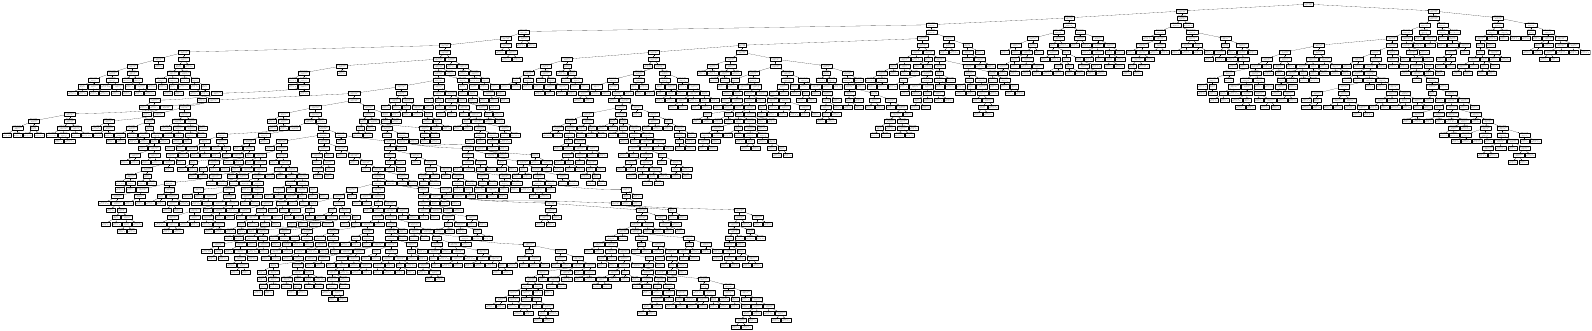
\includegraphics[width=\textheight,height=4cm]{ALL_BASELINE_1}
    \caption[all-baseline-1]{\textbf{BASELINE Set Decision Tree}: A
    decision tree trained using the \textbf{BASELINE} set.}
    \label{fig:all-baseline-1}

    \vspace{20mm}

    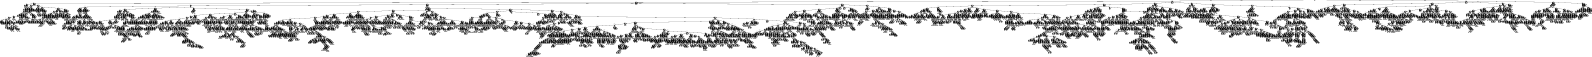
\includegraphics[width=\textheight,height=1cm]{ALL_ERROR_1}
    \caption[all-error-1]{\textbf{ERROR Set Decision Tree}: A highly
        overfit decision tree trained on the single parameter \textbf{ERROR}
        set. Each node forms an arbitrary decision on the \textbf{error-rate}
        parameter.}
    \label{fig:all-error-1}
\end{sidewaysfigure}
\begin{figure}[htbp!]
    \centering
    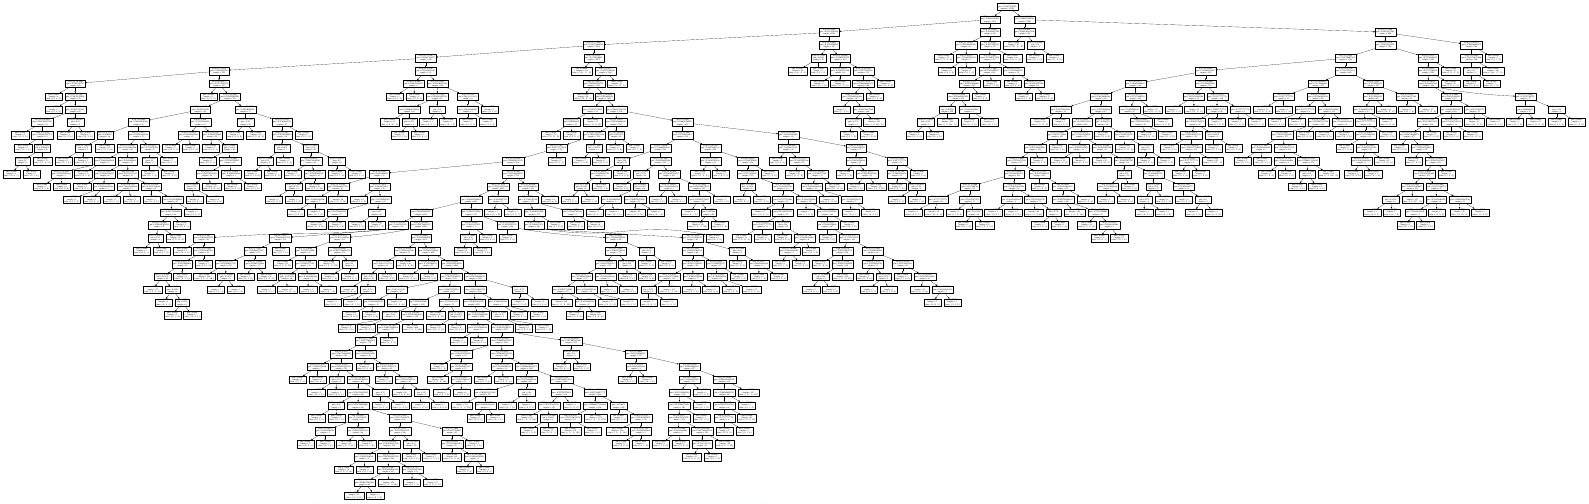
\includegraphics[width=1\textwidth]{ALL_AQC_1}
    \caption[all-aqc-1]{\textbf{AQC Set Decision Tree}: A more reasonably sized
    decision tree trained on the \textbf{AQC} set.}
    \label{fig:all-aqc-1}
\end{figure}
\begin{figure}[htbp!]
    \centering
    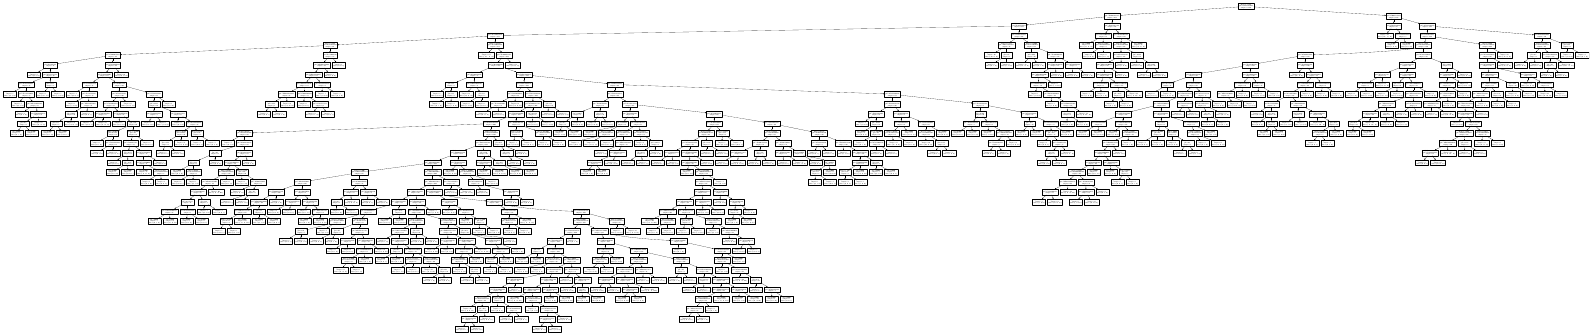
\includegraphics[width=1\textwidth]{ALL_AQC_2}
    \caption[all-aqc-1]{\textbf{AQC Set Decision Tree}: A more reasonably sized
    decision tree trained on the \textbf{AQC} set.}
    \label{fig:all-aqc-2}
\end{figure}

Figure~\ref{fig:all-error-1} is a highly overfit tree... and would require 42m
of A4!

\begin{figure}[htbp!]
    \centering
    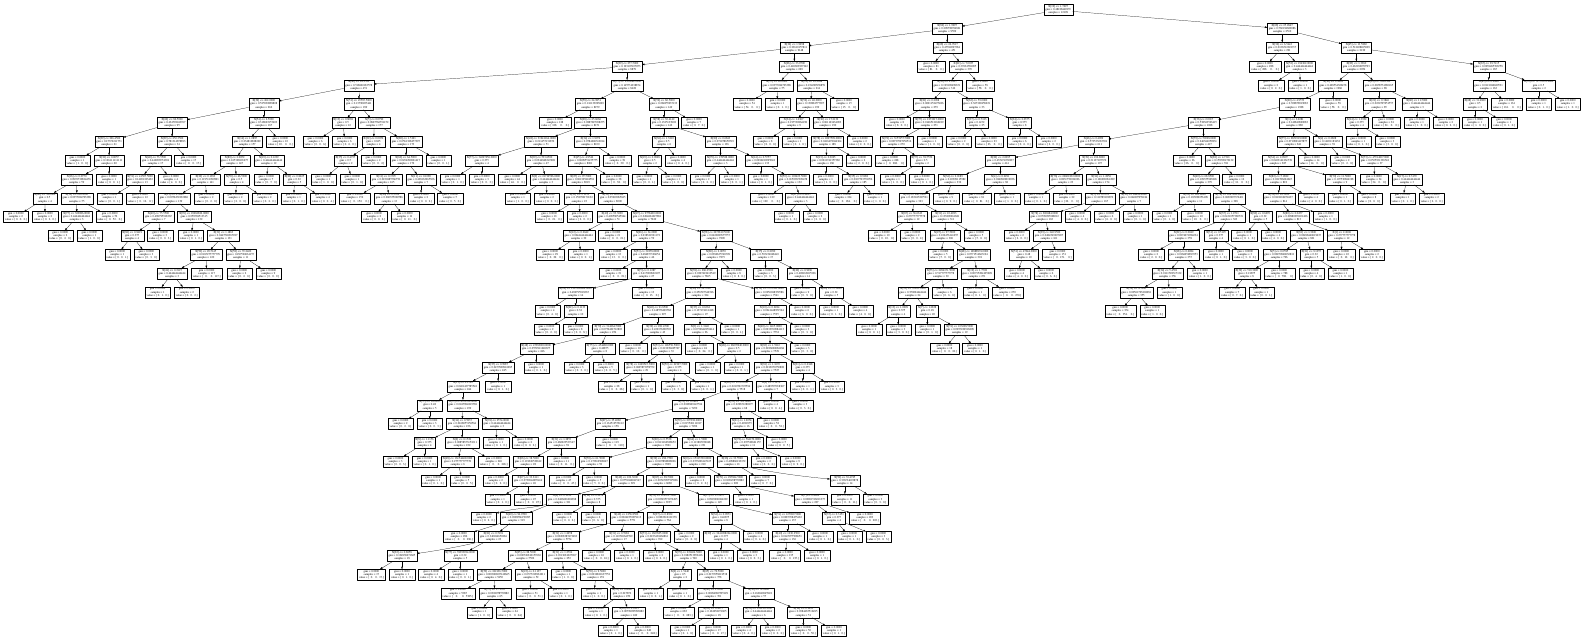
\includegraphics[width=1\textwidth]{ALL_ALL_1}
    \caption[all-all-1]{\textbf{ALL Set Decision Tree}: A more reasonably sized
    decision tree trained on the \textbf{ALL} set.}
    \label{fig:all-all-1}
\end{figure}
\begin{figure}[htbp!]
    \centering
    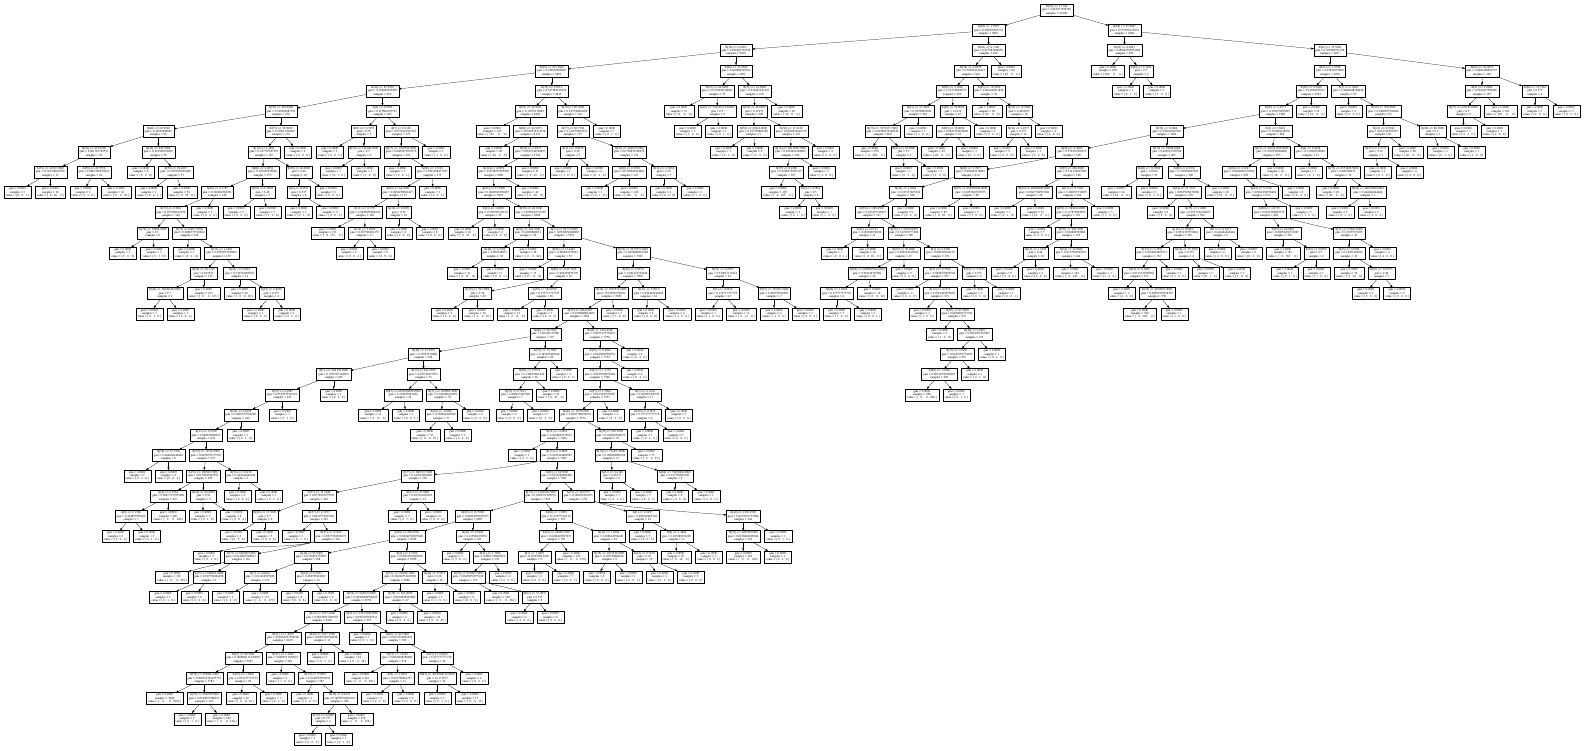
\includegraphics[width=1\textwidth]{ALL_ALL_2}
    \caption[all-all-2]{\textbf{ALL Set Decision Tree}: A more reasonably sized
    decision tree trained on the \textbf{ALL} set.}
    \label{fig:all-all-2}
\end{figure}


\section{Informed Parameter Selection}

Whilst the crude parameter sets of the previous section were useful to gain
understanding of the data that we have, it was necessary to obtain more
deliberate decisions for parameters to utilise in the model.

...important to find the "best" parameters
...what is best? scikit-learn uses total gini information

...frontier uses two methods:
\begin{itemize}
    \item Backward elimination; pruning parameters with the lowest total gini
    \item Call scikit-learn's SelectKBest
\end{itemize}

\begin{listing}[H]
    \caption[frontier-warnings]{\textbf{Frontier Variance Warnings}:
        Warnings issued for \textbf{auto\_qc} parameters that have been found to
        have no variance by one of \textbf{Frontier}'s sanity checking procedures.}
    \label{list:frontier-warnings}
    \begin{minted}[mathescape,
                %linenos,
                numbersep=5pt,
                gobble=0,
                frame=lines,
                framesep=2mm]{bash}
/pools/encrypted/sanger/frontier/data/bamcheck_2013dec25_ratios_out/(13455 files)
[WARN] bases-trimmed parameter has 0 variance (with mean 0.00)
[WARN] filtered-sequences parameter has 0 variance (with mean 0.00)
[WARN] is-paired parameter has 0 variance (with mean 1.00)
[WARN] is-sorted parameter has 0 variance (with mean 1.00)
[WARN] maximum-length parameter has 0 variance (with mean 100.00)
[WARN] non-primary-alignments parameter has 0 variance (with mean 0.00)
[WARN] quality-dropoff-high-iqr-threshold parameter has 0 variance (with mean 10.00)
[WARN] quality-dropoff-ignore-edge-cycles parameter has 0 variance (with mean 3.00)
[WARN] quality-dropoff-runmed-k parameter has 0 variance (with mean 25.00)
    \end{minted}
\end{listing}

Parameters with no variance will have constant value across all observations
regardless of their class label and will thus be unhelpful in predicting class
membership for future observations. Such parameters can be safely discarded,
Listing~\ref{list:frontier-warnings} displays warnings issued by
\textbf{Frontier} for several of the \textbf{auto\_qc}
\subsection{Parameter Selection}

\section{Trees}
\subsection{Application of Best Practice}
...scikit has no post pruning...

\textbf{DecisionTreeClassifier} accepts the following optional arguments upon
concstruction:

\begin{itemize}
    \item \textbf{max\_depth} \hfill\\
        Prevent the tree from growing beyond a specified depth.
    \item \textbf{min\_samples\_split} \hfill\\
        Prevent a node in the tree from being split further if it does not
        contain enough observations.
    \item \textbf{min\_samples\_leaf} \hfill\\
        Prevent a node in the tree from being split further if it would create a
        leaf smaller than the required minimum.
\end{itemize}

\subsection{Initial Trees}

\subsection{Ignoring Warnings}

\subsubsection{Cross Validation}

...method in which to measure classification accuracy...
...potentially use a weighting to penalise mistakes in smaller classes...

...K fold cross validation
...using stratified K fold cross validation...

\subsubsection{Confusion Matrices}
"Normal" confusion matrix and "Warnings" confusion matrix...

...
...

* incorrect degrees of freedom
* warnings: /usr/lib64/python2.7/site-packages/sklearn/feature\_selection/univariate\_selection.py:256: RuntimeWarning: invalid value encountered in divide, causing NaN
* Replaced univariate\_selection with version from master
* needed use force np.float64
* ...actually data was 0... gg

